\documentclass{hw}

\usepackage{stmaryrd}

\providecommand{\F}{\ensuremath{\mathbb{F}}}

\usepackage{tikz}
\usetikzlibrary{automata,positioning}

\begin{document}
\hwheader{15-354}{Computational Discrete Mathematics}{Fall 2018}{Synchronous Model Checking}{Uday Shankar}{us@andrew.cmu.edu}

\section*{Usage}
\subsection*{Defining an automaton}
In this package, an automaton contains information about the names of the tapes it reads from.
This means, for instance, that $x \rightarrowtriangle z$ and $y \rightarrowtriangle z$ are
distinct automata, even though the relation $\rightarrowtriangle$ is the same in both.
As such, we suggest defining an automaton as a function from tape names to an \code{Automaton}
object, or, in our case, a suspension of an \code{Automaton} object. Here is an example
for the successor automaton.
\begin{center}
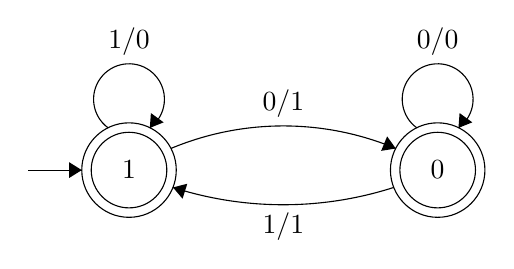
\begin{tikzpicture}[scale=0.2]
\tikzstyle{every node}+=[inner sep=0pt]
\draw [black] (52.2,-29.6) circle (3);
\draw (52.2,-29.6) node {$0$};
\draw [black] (52.2,-29.6) circle (2.4);
\draw [black] (32.6,-29.6) circle (3);
\draw (32.6,-29.6) node {$1$};
\draw [black] (32.6,-29.6) circle (2.4);
\draw [black] (26.2,-29.6) -- (29.6,-29.6);
\fill [black] (29.6,-29.6) -- (28.8,-29.1) -- (28.8,-30.1);
\draw [black] (35.263,-28.226) arc (112.65918:67.34082:18.526);
\fill [black] (49.54,-28.23) -- (48.99,-27.46) -- (48.61,-28.38);
\draw (42.4,-26.3) node [above] {$0/1$};
\draw [black] (49.412,-30.702) arc (-72.17614:-107.82386:22.909);
\fill [black] (35.39,-30.7) -- (36,-31.42) -- (36.3,-30.47);
\draw (42.4,-32.3) node [below] {$1/1$};
\draw [black] (50.877,-26.92) arc (234:-54:2.25);
\draw (52.2,-22.35) node [above] {$0/0$};
\fill [black] (53.52,-26.92) -- (54.4,-26.57) -- (53.59,-25.98);
\draw [black] (31.277,-26.92) arc (234:-54:2.25);
\draw (32.6,-22.35) node [above] {$1/0$};
\fill [black] (33.92,-26.92) -- (34.8,-26.57) -- (33.99,-25.98);
\end{tikzpicture}
\end{center}
\begin{lstlisting}
def auto_succ(v1, v2):
    d = {
        "alphabet": frozenset(["0", "1"]),
        "initial": frozenset([1]),
        "adjlist": {
            1: {
                "final": True,
                "edges": [
                    (0, {v1: "0", v2: "1"}),
                    (1, {v1: "1", v2: "0"})
                ]
            },
            0: {
                "final": True,
                "edges": [
                    (1, {v1: "1", v2: "1"}),
                    (0, {v1: "0", v2: "0"})
                ]
            }
        }
    }
    def susp(debug=0):
        if debug > 1:
            print("Auto_succ", d)
        return Automaton(d)
    return susp
\end{lstlisting}
The dictionary should be fairly understandable - at the top level, we store
the alphabet, set of initial states, and an adjacency list to store the
underlying graph. Edges are tuples of the form $(v, l)$ where $v$ is the
destination vertex, and $l$ is a dictionary that maps the tape name to the
character expected on that tape. The rest of the syntax involved
in building an automaton is boilerplate and can be copy-pasted.
Please do make sure that all edge labels in your automaton are complete,
in the sense that all the dictionaries that represent your labels should
have the same set of keys.

\subsection*{Writing formulae}
Once the atomic formulae are defined (via automata), building first-order formulae
is easy. The syntax is self-explanatory. For example, if we use $\rightarrowtriangle$
to represent the successor relation, we can express injectivity, i.e. the formula
$$(\forall x)(\forall y)(\forall z)(x \rightarrow z \wedge y \rightarrow z \implies x = y)$$
as
\begin{lstlisting}
ForAll("x", ForAll("y", ForAll("z", Implies(And(auto_succ("x", "z"),
auto_succ("y", "z")), auto_eq("x", "y")))))
\end{lstlisting}
The amount of computation performed when the formula is constructed is minimal.
Actual evaluation of the formula is done by calling the \code{Eval} function. Note that
this will throw an exception if the input formula is not a sentence.
For a full list of the available constructors of first-order formulae, see \code{formulae.py}.

\subsection*{Debugging level}
You can pass a keyword argument called \code{debug} to \code{Eval} to change
verbosity. The default is $0$ which prints nothing. If you pass $1$, it will print
the computations being performed and the size of the automaton at each step. If
you pass $2$, it will print everything included in $1$ along with all intermediate automata.

\subsection*{Cellular Automata}
Some of the tests included in \code{tests.py} involve model checking on
cellular automata. As written, they run on the rule 90 cellular automaton,
but this is easy to change. The function \code{rho90} in \code{tests.py} contains the definition
of the rule 90 cellular automaton, but you can change it to a different rule.
The tests will update automatically.

\subsection*{Putting it all together}
To try it yourself, we recommend you edit \code{tests.py} directly. There are a few useful
automata already defined there for your use, and a few examples that you can use to learn
the syntax. You should then be able to run \code{tests.py} using Python 3, or by just doing
\code{./tests.py}.
Hopefully everything works.

\section*{Implementation details}
\subsection*{Organization}
\code{automata.py} contains the routines that actually manipulate the machines. \code{tests.py}
contains some actual automata and some tests. \code{formulae.py} contains wrapper functions
for the routines in \code{automata.py} that are more readable and support lazy evaluation.

\subsection*{Algorithms}
In order to process first-order formulae, in addition to dealing with the atomic
formulae (in this context, defined via synchronous automata), we need to be able
to handle the inductive constructors (quantifiers and boolean connectives). We
discuss briefly how these are implemented. All functions mentioned are in \code{automata.py}.

\begin{enumerate}
  \item (Disjunction) If our formula is of the form $A \vee B$ and we have automata
  $\mathcal{A}$ and $\mathcal{B}$ representing $A$ and $B$ respectively, we need to compute
  an automaton representing $A \vee B$. Since we allow for nondeterminism, this is easy
  - we just take the union of the automata $\mathcal{A}$ and $\mathcal{B}$ and make
  the set of initial states the union of the initial states in $\mathcal{A}$ and the initial
  states in $\mathcal{B}$. The actual code, implemented in \code{disj}, does this and a bit
  of pruning that is necessary to maintain invariants.
  \item (Conjunction)  If our formula is of the form $A \wedge B$ and we have automata
  $\mathcal{A}$ and $\mathcal{B}$ representing $A$ and $B$ respectively, we need to compute
  an automaton representing $A \wedge B$. For this we use the classic product construction,
  where we take the product of the state sets of $\mathcal{A}$ and $\mathcal{B}$ and simulate
  both in parallel. The naive way of doing this is quite wasteful, however, as many of
  the elements of this product are inaccessible from the initial states. As such, we
  instead compute a closure under transitions of the initial state set. That is, if $I_{\mathcal{A}}$
  and $I_{\mathcal{B}}$ are the initial state sets, we compute $\mathrm{Clos}(I_{\mathcal{A}} \times I_{\mathcal{B}}, \Delta)$
  where $\Delta: Q_{\mathcal{A}} \times Q_{\mathcal{B}} \times \Sigma \to \mathcal{P}(Q_{\mathcal{A}} \times Q_{\mathcal{B}})$
  ($\Sigma$ is the set of all labels) via
  $$\Delta(p, q, \sigma) = \delta_{\mathcal{A}}(p, \sigma) \times \delta_{\mathcal{B}}(q, \sigma)$$
  This helps a lot to keep the automaton size down, which keeps our algorithms somewhat fast. The
  implementation of the closure algorithm is located in \code{product}, and the entire conjunction algorithm
  is in \code{conj}.
  \item (Negation) Since we allow for nondeterminism, there is no straightforward way to
  negate an automaton without first determinizing. As usual, determinization is a potentially
  exponentially-expensive process, but we make it fairly fast in all but the most bizarre
  cases by using a closure algorithm similar to the one shown above. That is, instead of using
  the full powerset as the state set of the determinized automata, we start with the initial
  state set and only move to those elements of the powerset that are strictly needed.
  This is an extremely important optimization for many reasons. First, it makes the algorithm
  actually run in time (at least on the simple test cases we tested) - even just a couple
  full determinizations on an automaton with $5$ states can and will blow it up. Second,
  the closure-based algorithm makes it so that if we perform two determinizations consecutively
  (which happens often when we have a bunch of universal quantifiers), the second is much
  cheaper than the first. The determinization code is found in \code{determinize}, and the
  small amount of extra code needed for negation can be found in \code{neg}.
  \item (Existential Quantifier) Nondeterminism allows for an easy solution to reducing
  formulae of the form $(\exists x)(A(x))$ - just erase the $x$ track from the automaton
  representing $A$. This is fast and so no optimization was considered. The code is in \code{exists}.
\end{enumerate}

All other first-order formula constructors are implemented as macros in terms
of these basic functions; see \code{formulae.py} for details on how this works.

We additionally considered optimizations involving running minimization algorithms after
determinization made the automaton blow up too large, but we did not have time to implement them.

\subsection*{Weird annoyances}
If you look at the key functions in \code{automata.py}, you might find some unnatural-looking
stuff that deals with propositional logic directly. From experimentation, we found that
in some cases, a fully erased automaton (unlabeled edges) did not play nice with
the boolean connectives. We address this by immediately reducing to a boolean value and
throwing out the automaton when
the last track is erased, and then special casing in the functions that process boolean
connectives.

\subsection*{Known Bugs}
For some reason, the clearly true formula $(\forall x)(\exists y)(x \neq y)$
evaluates to false. We aren't sure why this is, but we believe that it has something
to do with the empty string - for every other string, there is a string of the same
length that is not equal to it, but this does not hold for the empty string.

\end{document}
